\documentclass[12pt,a4paper]{article}
\usepackage{needspace}
\usepackage{tocloft}

\usepackage{graphicx}

\usepackage{tocloft}
\renewcommand{\cftfigpresnum}{FIGURA }
\renewcommand{\cftfigaftersnum}{ : }
\setfloatlink{}
\addtolength{\cftfignumwidth}{3em} 

\usepackage[utf8]{inputenc}
\usepackage[T1]{fontenc}
\usepackage[brazil]{babel}
\usepackage{graphicx}
\usepackage{geometry}
\geometry{left=3cm,right=2cm,top=3cm,bottom=2cm}
\renewcommand{\baselinestretch}{1.5}
\usepackage{mathptmx}
\usepackage{hyperref}
\hypersetup{colorlinks=true, linkcolor=black, urlcolor=blue}
\usepackage{fancyhdr}
\pagestyle{fancy}
\setlength{\headheight}{15pt}
\fancyhf{}
\rhead{\thepage}
\renewcommand{\headrulewidth}{0pt}
\usepackage{needspace}
\begin{document}
\pagenumbering{arabic}
\setcounter{page}{1}
\widowpenalty=10000
\hyphenpenalty=10000
\exhyphenpenalty=10000
\sloppy


% ============ CAPA ============
\begin{titlepage}
\centering
% \vspace*{1cm}
{\large\bfseries UNIVERSIDADE VIRTUAL DO ESTADO DE SÃO PAULO\par}
\vspace{2cm}
{\normalsize Jessica Fabiane Costa de Medeiros\par}
{\normalsize Luiz Henrique Ferreira Silva\par}
{\normalsize Mikael Silva\par}
{\normalsize Rafael Massao Okumura\par}
{\normalsize Thainá Alzira Carvalho Vieira Batista\par}
{\normalsize Willian Pires da Silva\par}
\vspace{2.5cm}
{\large\bfseries Tintas MGMT: Sistema de Organização e\par}
\vspace{0.3cm}
{\large\bfseries Análise de Dados Empresarial\par}
\vspace{3cm}
\fbox{\parbox{\textwidth}{
\centering
\textbf{Vídeo de apresentação do Projeto Integrador}\\[0.3cm]
<link>
}}
\vfill
{\large Araçariguama, Iperó, Itapetininga, Salto - SP\par}
{\large 2026\par}

\end{titlepage}
\pagestyle{empty}

% ============ FOLHA DE ROSTO ============
\pagebreak
\thispagestyle{empty}
\begin{center}
% \centering
% \vspace*{1cm}
{\large\bfseries UNIVERSIDADE VIRTUAL DO ESTADO DE SÃO PAULO\par}
\vspace{2cm}
\vspace{2.5cm}
{\large\bfseries Tintas MGMT: Sistema de Organização e\par}
\vspace{0.3cm}
{\large\bfseries Análise de Dados Empresarial\par}
\vspace{3cm}
{\linespread{1}\selectfont\leftskip=7cm   Relatório Técnico-Científico apresentado na disciplina de Projeto Integrador para o curso de Bacharelado em Tecnologia da Informação, Ciência de Dados e Engenharia de Computação da Universidade Virtual do Estado de São Paulo (UNIVESP).\par}
% \\[1.2cm]
\vfill
{\large Araçariguama, Iperó, Itapetininga, Salto - SP\par}
{\large 2026\par}
\end{center}

% ============ RESUMO ============
\clearpage
\thispagestyle{empty}

{\centering
Jessica Fabiane Costa de Medeiros; Luiz Henrique Ferreira Silva; Mikael Silva; Rafael Massao Okumura; Thainá Alzira Carvalho Vieira Batista; Willian Pires da Silva\\[0.3cm]
Tintas MGMT: Sistema de Organização e Análise de Dados Empresarial\\[0.3cm]
Relatório Técnico-Científico\\[0.3cm]
Curso de Bacharelado em Tecnologia da Informação, Ciência de Dados e Engenharia de Computação\\[0.3cm]
Tutora: Kelly de Santana Santana\\[0.3cm]
2026\par}
\vspace{1cm}

\section*{Resumo}

{\linespread{1}\selectfont\setlength{\baselineskip}{12pt}
A operação de uma fábrica de tintas envolve compra de matérias-primas, produção, envase, armazenamento, venda e manutenção de equipamentos. Quando essas informações não são registradas de forma organizada, torna-se difícil acompanhar a quantidade produzida, o volume vendido, os tamanhos de embalagem mais procurados, as cores de maior saída, os níveis de estoque, as perdas e as paradas de máquinas. Essa dificuldade prejudica o planejamento da produção e a tomada de decisões da empresa. Com base no levantamento inicial realizado junto a uma fábrica de tintas, este trabalho propõe o desenvolvimento do Tintas MGMT, um aplicativo web destinado à organização dos dados operacionais da empresa e à visualização dos resultados. A solução reúne informações sobre produção, vendas, estoque, perdas, atrasos e manutenção em uma estrutura única e de fácil consulta. O código-fonte está disponível em: https://github.com/RafaelMassao/TintasMGMT. O projeto está relacionado ao desenvolvimento de análise de dados e à preparação de uma interface para apresentação das informações. O desenvolvimento inicial contempla a definição do problema, o levantamento de requisitos, a criação da estrutura do aplicativo, o cadastro das informações básicas e a elaboração de wireframes das principais telas. A continuidade do projeto deverá permitir a substituição de registros dispersos por dados organizados, possibilitando análises mais precisas e melhorias no acompanhamento da operação.
\par}

\vspace{2cm}

\textbf{Palavras-chave:} Aplicativo web; análise de dados; fábrica de tintas; produção; estoque; manutenção; visualização de informações.

% ============ LISTA DE FIGURAS ============
\clearpage
\listoffigures

% ============ SUMÁRIO ============
\clearpage
\tableofcontents

% ============ CORPO ============
\clearpage
\pagestyle{fancy}
\section{INTRODUÇÃO}
\enlargethispage{-4\baselineskip}
A escolha deste tema surgiu a partir do contato com uma empresa do segmento de fabricação de tintas.

Durante as conversas iniciais, foram identificados elementos da operação de uma fábrica de tintas: a produção envolve compra de matérias-primas, envase, armazenamento, vendas e manutenção de equipamentos. Quando essas informações não são registradas de forma organizada, torna-se difícil acompanhar a quantidade produzida, o volume vendido, os tamanhos de embalagem mais procurados, as cores de maior saída, os níveis de estoque, as perdas e as paradas de máquinas. Essa dificuldade prejudica o planejamento da produção e a tomada de decisões da empresa.

Além disso, conhecer apenas a quantidade produzida não é suficiente para compreender o desempenho da fábrica. É necessário saber quais produtos foram fabricados, quais cores foram utilizadas, quais tamanhos de embalagem foram produzidos, quanto foi vendido, quais matérias-primas foram consumidas e quais equipamentos permaneceram parados.

A ausência de registros organizados pode dificultar o planejamento e fazer com que decisões importantes sejam tomadas com base apenas na memória ou em anotações separadas. Também pode dificultar a identificação de perdas e atrasos. Uma parada em um motor, uma falha na bomba ou uma revisão não realizada podem interferir na produção e no cumprimento dos prazos de entrega.

Nesse contexto, o presente trabalho concentra-se na concepção e no desenvolvimento inicial do Tintas MGMT, um aplicativo web voltado à organização dos dados de uma fábrica de tintas. A proposta é reunir informações relevantes da operação e apresentar os resultados de forma simples, permitindo que a empresa acompanhe sua produção, vendas, estoque e manutenção com maior clareza.
O projeto também se relaciona ao tema de desenvolvimento de análise de dados em escala utilizando conjuntos de dados existentes ou capturados por dispositivos e aprendizagem de máquina, preparando uma interface para visualização dos resultados. Nesta etapa, o foco está na organização da base de informações e na definição da interface. A utilização de dados históricos, sensores e modelos de análise deverá ocorrer conforme a aplicação evolua e conforme a empresa disponha de registros suficientes.

\clearpage
\section{DESENVOLVIMENTO}

\subsection{Objetivos}
\subsubsection*{Objetivo geral}
Desenvolver um aplicativo web capaz de organizar dados de produção, vendas, estoque, perdas, atrasos e manutenção de uma fábrica de tintas, permitindo visualizar as principais informações da operação e apoiando o planejamento da empresa.

\subsubsection*{Objetivos específicos}
\begin{itemize}
\item \textbf{Cadastros base —} Desenvolver cadastros base por meio de catálogos organizados onde serão registrados produtos, cores, embalagens, matérias-primas, fornecedores, equipamentos, tanques e clientes.
\item \textbf{Produção e vendas —} Desenvolver sistema de monitoramento de produção e vendas por meio de controle de lotes de produção e movimentações de estoque onde serão registradas entradas e saídas de produtos acabados.
\item \textbf{Perdas e atrasos —} Desenvolver registro de perdas e atrasos por meio de controle de paradas de máquinas onde serão registrados motivos e responsáveis com data.
\item \textbf{Manutenção —} Desenvolver organização de manutenção por meio de controle de revisões periódicas onde serão registrados equipamentos com QR code e paradas (preventiva e corretiva).
\item \textbf{Interface e indicadores —} Desenvolver interface e indicadores por meio de dashboard onde serão apresentados indicadores de produção, vendas, estoque e manutenção para apoio à decisão.
\item \textbf{Base de dados —} Preparar base de dados por meio de esquema relacional no Supabase com RLS onde serão organizados dados para futuras análises e sensores.
\end{itemize}

\subsection{Justificativa e delimitação do problema}
A fabricação de tintas depende da disponibilidade de materiais, equipamentos, mão de obra, embalagens e espaço para armazenamento. Uma falha em qualquer uma dessas etapas pode interferir na produção. Além disso, os produtos podem possuir diferentes cores, volumes e destinos, o que aumenta a necessidade de organizar os registros.

A informação de que a empresa produz aproximadamente 150 baldes por semana representa apenas uma visão geral. Para apoiar decisões, é necessário detalhar essa produção. Deve-se identificar quantos baldes correspondem às embalagens de 1 litro, 3,6 litros e 18 litros, quais cores são mais requisitadas, quais produtos permanecem em estoque e quais itens precisam ser repostos.

A mesma necessidade existe em relação às vendas. Saber o total vendido é importante, mas também é necessário observar o comportamento da demanda. Uma determinada embalagem pode possuir maior saída em um período, enquanto uma cor pode ser mais procurada em determinada época. A organização desses dados pode ajudar a empresa a planejar melhor suas compras e sua produção.

A manutenção também precisa ser considerada. A empresa realiza revisões periódicas, e os equipamentos possuem relação direta com a continuidade da produção. Registrar a data de uma revisão, o equipamento envolvido, o tipo de manutenção e o tempo de parada pode ajudar a compreender a origem de atrasos e perdas.

A justificativa social e econômica deste projeto está relacionada à possibilidade de apoiar uma empresa real na organização de suas atividades. Um sistema simples e centralizado pode facilitar a consulta de informações, reduzir a dependência de registros dispersos e contribuir para decisões mais seguras. A solução também pode apoiar o crescimento da empresa, pois uma base organizada facilita a identificação de necessidades e oportunidades.

A justificativa cultural está relacionada à preservação do conhecimento operacional acumulado nas fábricas de tintas da região de Araçariguama, Iperó, Itapetininga e Salto (SP). Essas fábricas de pequeno e médio porte operam historicamente com registros em papel, planilhas dispersas e controles de memória, sem integração entre produção, vendas, estoque e manutenção. A ausência de ferramentas simples e acessíveis de organização de dados representa um risco à preservação desse saber, que se perde com a rotatividade de pessoal e a aposentadoria de operadores experientes. O Tintas MGMT contribui para a sistematização desse conhecimento acumulado, centralizando dados em um único repositório digital acessível a todos os perfis de usuário. Além disso, apoia o desenvolvimento socioeconômico da região ao permitir que pequenas fábricas de tintas ganhem em rastreabilidade, redução de perdas e tomada de decisão baseada em dados, sem a necessidade de investir em sistemas ERP complexos e de alto custo.

A justificativa acadêmica deste trabalho está relacionada à aplicação de conhecimentos de desenvolvimento web, banco de dados, organização da informação, análise de dados e visualização. O trabalho permite estudar um problema real e transformá-lo em uma proposta tecnológica, passando pelas etapas de levantamento, definição de requisitos, modelagem, construção de protótipo e avaliação inicial.

Estudos relacionados apontem que sistemas MES/ERP para PMEs são complexos, caros e representam um exagero para fábricas de pequeno porte \parencite{SILVA2020}. A Manufatura 4.0 foca em grandes indústrias com sensores IoT, sem abordar a organização básica de dados \parencite{FERNANDES2019}. Já a análise de dados em PMEs apresenta uma lacuna entre "ter dados" e "usar dados", em decorrência da falta de ferramenta acessível \parencite{SOARES2021}.

O Tintas MGMT preenche essa lacuna ao propor uma solução web simples, de baixo custo e com implantação gratuita (Vercel + Supabase, plano gratuito), focada na organização dos dados antes de análises avançadas. A proposta estabelece uma base para futuro aprendizado de máquina e integração de sensores, possui RBAC nativo para separação de responsabilidades (produção, vendas, estoque, manutenção) e é extensível: o schema do Supabase permite adicionar sensores e ML sem refatorar o frontend.

Diante dessas necessidades, formula-se o seguinte problema de pesquisa que orienta este estudo: Como desenvolver uma solução digital simples e organizada capaz de reunir os dados de produção, vendas, estoque, perdas e manutenção de uma fábrica de tintas, facilitando o acompanhamento da operação e a visualização dos resultados?

A delimitação do problema concentra-se no desenvolvimento inicial de um aplicativo web para uso interno da empresa. O protótipo contempla a estrutura de acesso, os cadastros básicos, a organização das áreas do sistema e a definição das principais telas. Nesta etapa, os módulos de produção, pedidos, estoque, perdas, manutenção e relatórios ainda não estão completamente finalizados. Também não fazem parte do escopo inicial a automação direta das máquinas, a emissão fiscal, a integração contábil ou a implantação imediata de sensores.

\subsection{Contribuições para o Público Externo}
As contribuições do projeto Tintas MGMT estendem-se além da empresa beneficiária, impactando a comunidade e o ambiente acadêmico:

\begin{enumerate}
\item \textbf{Contribuições para a Empresa Beneficiária}
O sistema proposto traz benefícios concretos para a fábrica de tintas:

\begin{itemize}
\item Centralização de dados: Substitui cadernos, planilhas e anotações dispersas por uma base única e organizada, garantindo que todas as informações estejam em um único local de fácil consulta.
\item Rastreabilidade completa: É possível acompanhar a produção desde o recebimento das matérias-primas até a entrega dos produtos acabados, incluindo lotes, cores, embalagens e quantidades.
\item Tomada de decisão mais segura: Com dados organizados e indicadores claros, a gestão pode tomar decisões mais embasadas sobre compras, produção e manutenção, reduzindo a dependência da memória ou de anotações isoladas.
\end{itemize}

\item \textbf{Contribuições Socioeconômicas}
\begin{itemize}
\item Apoio a empresas reais: O sistema simples e centralizado facilita a consulta de informações, reduz a dependência de registros dispersos e contribui para decisões mais seguras.
\item Identificação de perdas e ganhos: O sistema registra perdas, atrasos e motivos, permitindo identificar quais etapas do processo apresentam maiores desvios e oportunidades de melhoria.
\item Suporte ao crescimento: Uma base de dados organizada facilita a identificação de necessidades e oportunidades, suportando o crescimento da empresa ao longo do tempo.
\end{itemize}

\item \textbf{Contribuições Acadêmicas e Técnicas}
\begin{itemize}
\item Aplicação de conhecimentos: O trabalho aplica conhecimentos de desenvolvimento web, banco de dados, organização da informação, análise de dados e visualização para criar uma solução tecnológica a partir de um problema real.
\item Desenvolvimento sustentável: A proposta foca em criar uma solução simples e adequada ao problema identificado, sem perder a possibilidade de evolução para análises mais avançadas no futuro (sensores, aprendizado de máquina, automação).
\item RBAC nativo: O sistema possui controle de acesso por usuário e perfis de utilização, garantindo que diferentes áreas (produção, vendas, estoque, manutenção) tenham acesso apenas às informações relevantes.
\end{itemize}
\end{enumerate}

\subsection{Fundamentação teórica}

As disciplinas do curso de Tecnologia da Informação, Ciência de Dados e Engenharia de Computação da UNIVESP proporcionaram os conhecimentos técnicos necessários para a construção do Tintas MGMT. A seguir, descreve-se a aplicação de cada disciplina ao longo do projeto:

\textbf{Análise de Dados}: As disciplinas de análise de dados capacitaram a transformação de registros operacionais em informações significativas. No contexto do Tintas MGMT, os conceitos de limpeza, organização e exploração de dados foram aplicados para estruturar bases de informações sobre produção, vendas, estoque e manutenção. A análise possibilita identificar padrões de consumo, comportamentos de demanda e oportunidades de otimização, fundamentando a tomada de decisões baseada em evidências rather do que da memória ou anotações isoladas.

\textbf{Banco de Dados}: O conhecimento em modelagem e administração de bancos de dados foi essencial para estruturar o schema do Supabase utilizado no projeto. Aplicou-se o conceito de relações relacionais (Elmasri & Navathe, 2019) para organizar entidades como produtos, cores, embalagens, matérias-primas, fornecedores, equipamentos, tanques e motivos de perda, garantindo consistência, integridade e evititação de redundância de dados. O schema foi desenhado para ser extensível, permitindo a adição de sensores e modelos de aprendizado de máquina no futuro sem refatoração do frontend.

\textbf{Desenvolvimento Web}: As disciplinas de desenvolvimento web forneceram os fundamentos para construção da aplicação full-stack Tintas MGMT. A arquitetura implementou tecnologias modernas (React 19, TypeScript, TanStack Router, TanStack Start, Tailwind CSS v4, Radix UI) seguindo boas práticas de código mantenível, acessibilidade e separação de responsabilidades. A aplicação web foi desenvolvida com abordagem responsive e progressive enhancement, garantindo funcionalidade em diferentes dispositivos e níveis de familiaridade do usuário com ferramentas digitais.

\textbf{Indústria 4.0 e Manufatura}: Os conceitos de Indústria 4.0 foram estudados para entender o contexto atual da automação e integração de sistemas industriais. O Tintas MGMT adota uma abordagem graduada: inicia-se com a organização básica de dados antes de integrar sensores avançados ou automação de máquinas, conforme estudos relacionados apontam que sistemas MES/ERP para PMEs são complexos e caros, representando um exagero para fábricas de pequeno porte. A proposta preenche lacuna identificada entre "ter dados" e "usar dados" em PMEs, focando primeiro na estruturação da base antes de avançadas análises preditivas.

\textbf{Usabilidade e Design Centrado no Usuário}: As disciplinas de usabilidade e design de interação fundamentaram a criação de interfaces acessíveis e intuitivas. Princípios de Nielsen (1994) sobre simplicidade, clareza e facilidade de aprendizagem foram aplicados no design dos wireframes e na interface do Tintas MGMT. Norman (2013) sobre design centrado no usuário orientou a organização das informações para diferentes perfis (produção, vendas, estoque, manutenção), garantindo que cada área acesse apenas os dados relevantes por meio do RBAC nativo do sistema.

\textbf{Segurança da Informação}: O conhecimento em segurança da informação foi aplicado no planejamento de controle de acesso e proteção de dados. As diretrizes do OWASP Top 10 orientaram o planejamento de autenticação, controle de acesso e proteção contra exposição inadequada de informações. O sistema foi desenvolvido com RBAC (Role-Based Access Control) nativo, garantindo separação de responsabilidades entre as áreas de produção, vendas, estoque e manutenção, com perfis de usuário que restringem acesso às informações necessárias para cada função.

\textbf{Metodologia de Pesquisa}: As disciplinas de metodologia de pesquisa fundamentaram o estruturante do trabalho com as três etapas: Ouvir e Interpretar o Contexto, Criar / Prototipar e Implementar / Testar. Esse enfoque metodológico, caracterizado como pesquisa aplicada, permitiu desenvolver uma solução para um problema identificado em empresa real, com caráter exploratório (once the factory process is still being detailed) e descritivo (buscando representar as principais atividades e informações envolvidas).

Dessa forma, o Tintas MGMT integra conhecimentos interdisciplinares do curso de Tecnologia da Informação, Ciência de Dados e Engenharia de Computação, aplicando-os de forma articulada para resolver o problema identificado na fábrica de tintas — a falta de organização dos dados operacionais — sem perder a possibilidade de evolução para análises mais avançadas no futuro, incluindo integração de sensores, aprendizado de máquina e automação gradual.

\subsection{Metodologia}
O presente trabalho adota uma metodologia de pesquisa aplicada com três etapas estruturantes:

\textbf{Ouvir e Interpretar o Contexto} — Etapa de levantamento do problema junto à fábrica de tintas. Foram realizadas entrevistas semiestruturadas com o pessoal operacional da fábrica, complementadas por observação direta dos processos de produção, envase, armazenamento e manutenção dos equipamentos. O perfil dos participantes incluiu operadores de linha de produção, responsáveis pela manutenção e gestão da fábrica, com experiência operacional de 1 a 10 anos na região de Araçariguama, Iperó, Itapetininga e Salto (SP). Durante as conversas foram identificados os equipamentos utilizados na produção (tanque de tinta com capacidade aproximada de 2.000 litros, três motores trituradores, bomba responsável pelo deslocamento da tinta, tanque para água e equipamento de envase manual), os tamanhos de embalagem (1 litro, 3,6 litros e 18 litros), a existência de estoque de matérias-primas e produtos acabados, as revisões periódicas e a necessidade de acompanhar vendas, perdas e atrasos. Essas informações demonstram que existe uma operação produtiva que pode ser acompanhada por meio de dados, mas conhecer apenas a quantidade produzida não é suficiente para compreender o desempenho da fábrica — é necessário saber quais produtos foram fabricados, quais cores foram utilizadas, quais tamanhos de embalagem foram produzidos, quanto foi vendido, quais matérias-primas foram consumidas e quais equipamentos permaneceram parados. A ausência de registros organizados pode dificultar o planejamento e fazer com que decisões importantes sejam tomadas com base apenas na memória ou em anotações separadas.

\textbf{Criar / Prototipar} — Etapa de organização da estrutura inicial do aplicativo e criação de wireframes. Foi desenvolvido um aplicativo web com telas de autenticação, painel principal, cadastros e áreas reservadas para produção, pedidos, estoque, perdas e manutenção. Foram previstos cadastros para unidades de medida, cores, embalagens, produtos, clientes, fornecedores, materiais, equipamentos, tanques e motivos de perda e atraso. Também foram definidos perfis de acesso para controlar as áreas que cada usuário poderá consultar ou alterar. O processo incluiu a elaboração dos wireframes como rascunhos de baixa fidelidade, utilizando contornos simples, campos, tabelas e áreas reservadas. Foram planejadas telas para dashboard, produção, estoque e manutenção, representando a organização das telas antes da definição do visual final. A estrutura inicial já contempla o cadastro de produtos, cores, embalagens, clientes, fornecedores, materiais, equipamentos e tanques. Também foram definidos perfis de usuário, permitindo que as áreas do sistema sejam relacionadas às responsabilidades de cada pessoa. Essa organização evita que os dados sejam inseridos sem padrão e facilita a construção dos indicadores. O dashboard foi planejado para apresentar uma visão geral da operação, com informações sobre produção, vendas, estoque e manutenção. Nesta etapa, os dados apresentados são demonstrativos e servem para avaliar a organização da interface. Eles não representam resultados reais da empresa. A substituição por dados reais deverá ocorrer depois da implementação das tabelas de produção, vendas, estoque e manutenção.

\textbf{Implementar / Testar} — Etapa de implantação do protótipo e validação. Inclui a criação dos registros de produção, pedidos, estoque, perdas e manutenção no sistema. A validação ocorre com a comparação entre os registros do sistema e as informações utilizadas pela empresa, verificando se as telas são compreensíveis e se os resultados correspondem à realidade da operação. 

O protótipo foi testado através de validação inicial com wireframes de baixa fidelidade apresentados ao pessoal operacional da fábrica (operadores de linha, responsáveis pela manutenção e gestão), com experiência de 1 a 10 anos na região de Araçariguama, Iperó, Itapetininga e Salto (SP). Foram coletados feedbacks sobre a disposição dos campos, clareza dos indicadores e organização dos módulos de produção, vendas, estoque e manutenção.

As principais devolutivas coletadas indicam que o sistema proposto é útil para organizar dados operacionais dispersos. As principais sugestões de melhoria sugeridas com base nesses testes incluem: (1) implementação de campos obrigatórios para garantir completude dos dados de produção, (2) criação de checklists de revisão para equipamentos com QR code, (3) adição de gatilhos automáticos quando o envase for concluído, e (4) expansão do sistema para incluir módulos de compras e alertas de manutenção. Os wireframes de baixa fidelidade foram bem recebidos como ponto de partida para o desenvolvimento da interface, embora os usuários tenham solicitado mais exemplos visuais e demonstrações interativas. Em geral, a solução foi validada como viável para reduzir a dependência de registros em papel e planilhas dispersas, permitindo um acompanhamento mais claro da operação da fábrica de tintas.

As principais dificuldades encontradas na transformação da operação em informações registradas pelo sistema podem ser mitigadas pelas seguintes estratégias:

\begin{table}[h]
\centering
\caption{Estratégias de mitigação das principais dificuldades}
\begin{tabular}{p{0.45\textwidth}p{0.45\textwidth}}
\hline
\textbf{Dificuldade} & \textbf{Estratégia de Mitigação} \\
\hline
Produção "150 baldes/semana" sem detalhe por embalagem, cor, produto e período & Formulário de lote com campos obrigatórios: produto, cor, embalagem, quantidade planejada e realizada, tanque, datas \\
\hline
Incerteza sobre quando o produto acabado entra no estoque & Gatilho ao finalizar envase (\texttt{envase.status = concluido}) $\rightarrow$ registro em \texttt{movimentacao\_estoque} tipo entrada + atualiza \texttt{saldos\_estoque} \\
\hline
Registro de perdas e consumo & Tela dedicada `/perdas` com tipos: processo, quebra embalagem, vencimento, contaminação, outro; campo `valor\_estimado` \\
\hline
Acompanhamento impreciso de máquinas e paradas & Cadastro de equipamentos com QR code; checklist de revisão; parada: equipamento, causa, início/fim, lote/pedido relacionado \\
\hline
Dados dispersos em papel e memória individual & Base única Supabase com RLS; cada perfil acessa apenas seu módulo; dashboard unifica indicadores \\
\hline
\end{tabular}
\label{tab:mitigacao}
\end{table}

Os wireframes apresentados nesta seção representam a primeira organização das telas. Foram construídos como rascunhos de baixa fidelidade para demonstrar os campos e informações necessários.

\begin{figure}[htbp]
\centering
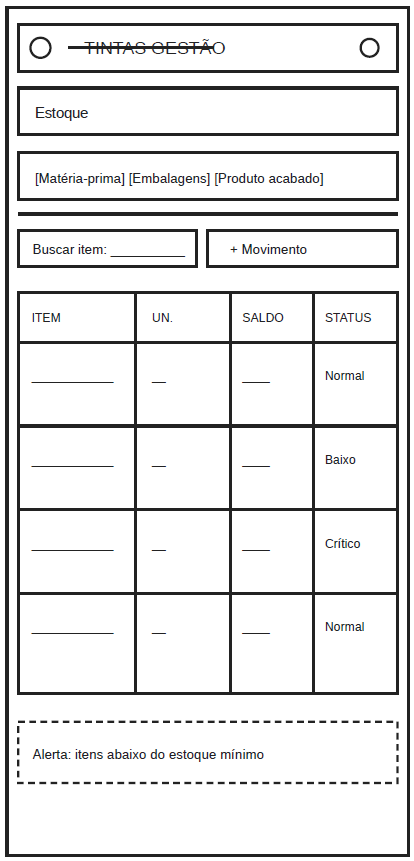
\includegraphics[width=0.35\textwidth]{figures/img1.png}
\caption[Wireframe Gestão]{Wireframe Gestão. Fonte: Elaboração própria, 2026}
\label{fig:gestao}
\end{figure}

A tela de Gestão permite a administração dos cadastros base da aplicação, incluindo produtos, cores, embalagens, matérias-primas, fornecedores, equipamentos, tanques e clientes. Cada cadastro possui campos para identificação, descrição e status, permitindo que o usuário organize as informações básicas antes de iniciar os registros operacionais.

\begin{figure}[htbp]
\centering
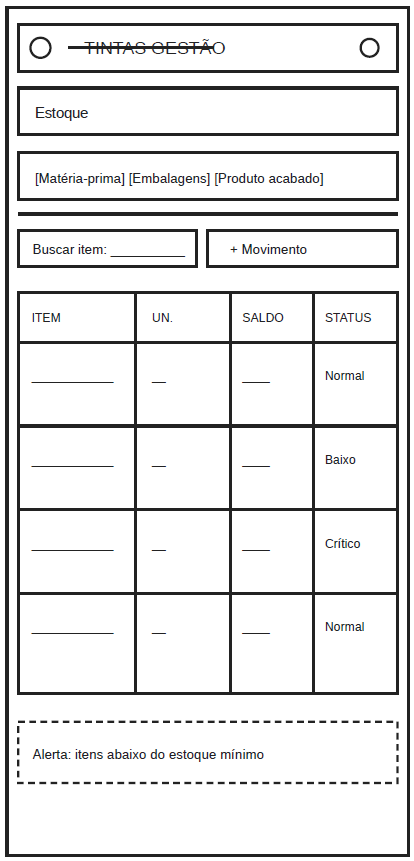
\includegraphics[width=0.35\textwidth]{figures/img2.png}
\caption[Wireframe Estoque]{Wireframe Estoque. Fonte: Elaboração própria, 2026}
\label{fig:estoque}
\end{figure}

A tela de Estoque apresenta os itens cadastrados com seus respectivos saldos. Possui funcionalidades para visualizar itens abaixo do estoque mínimo, registrar movimentações de entrada e saída, e acompanhar o rastreamento de lotes desde a produção até a entrega.

\begin{figure}[htbp]
\centering
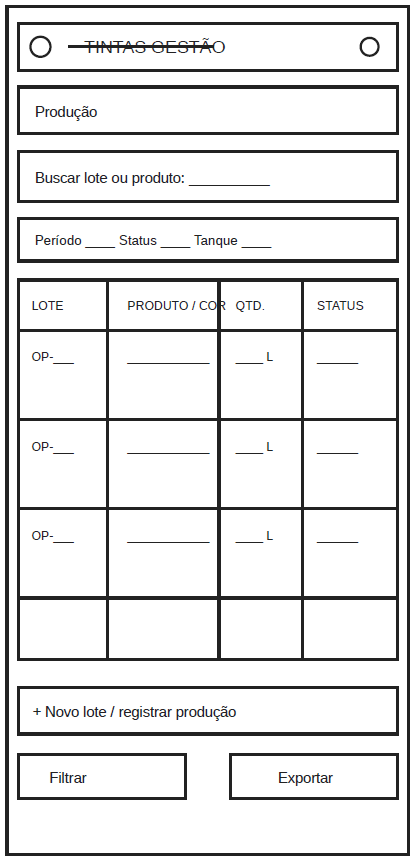
\includegraphics[width=0.35\textwidth]{figures/img3.png}
\caption[Wireframe Tela de Produção]{Wireframe Tela de Produção. Fonte: Elaboração própria, 2026}
\label{fig:producao}
\end{figure}

A tela de Produção permite controlar lotes de produção, pedidos e movimentações de estoque. Possui campos para registrar o produto, cor, embalagem, quantidade planejada e realizada, tanque utilizado e datas de início e fim do lote.

\begin{figure}[htbp]
\centering
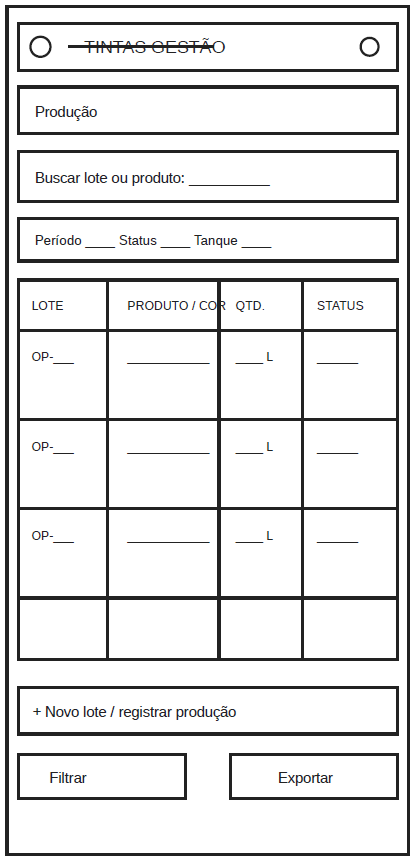
\includegraphics[width=0.35\textwidth]{figures/img4.png}
\caption[Wireframe Manutenção]{Wireframe Manutenção. Fonte: Elaboração própria, 2026}
\label{fig:manutencao}
\end{figure}

A tela de Manutenção organiza revisões periódicas, equipamentos com QR code e controle de paradas (preventiva e corretiva). Possui campos para registrar o equipamento envolvido, tipo de manutenção, data, causa, período de parada e responsável.

\subsubsection{Arquitetura da Solução}
O aplicativo foi desenvolvido com tecnologias web modernas, seguindo uma arquitetura full-stack:

\begin{itemize}
\item \textbf{Frontend:} React 19 com TypeScript, utilizando TanStack Router para roteamento baseado em arquivos e TanStack Start para renderização no servidor (SSR). Para estilização, utiliza Tailwind CSS v4 com componentes acessíveis do Radix UI. A visualização de dados é feita com Recharts, e formulários com validação são construídos com React Hook Form e Zod.
\item \textbf{Banco de dados e Backend:} Supabase (PostgreSQL + Auth + Real-time) com Row Level Security (RLS) para controle de acesso por perfil de usuário.
\item \textbf{Estrutura de rotas:} Inclui módulos para login, cadastro, dashboard, cadastros, produção, pedidos, estoque, envase, compras, perdas, manutenção, atrasos, alertas, relatórios e configurações.
\item \textbf{Perfis de acesso:} administrador, gestor, produção, estoque, vendas e manutenção.
\end{itemize}

De modo geral, o Tintas MGMT possui uma estrutura inicial capaz de receber os dados da empresa e transformá-los em informações organizadas, representando um primeiro passo para a criação de uma solução de acompanhamento operacional.

\clearpage
\section{RESULTADOS: SOLUÇÃO FINAL}

O grupo demonstrou a criação de soluções com base na metodologia indicada pela UNIVESP, respeitando os passos Ouvir, Criar e Implementar. Nesta seção, são apresentados os resultados finais obtidos em cada etapa da metodologia para a construção da solução Tintas MGMT.

\subsection{Solução adotada}
O Tintas MGMT é um aplicativo web full-stack desenvolvido com React 19 e TypeScript, utilizando TanStack Router para roteamento baseado em arquivos e TanStack Start para renderização no servidor (SSR). A estilização utiliza Tailwind CSS v4 com componentes acessíveis do Radix UI, e a visualização de dados é feita com Recharts. Os formulários possuem validação construída com React Hook Form e Zod. O backend utiliza Supabase (PostgreSQL + Auth + Real-time) com Row Level Security (RLS) para controle de acesso por perfil de usuário. A estrutura de rotas inclui módulos para login, cadastro, dashboard, cadastros, produção, pedidos, estoque, perdas, manutenção, atrasos, alertas, relatórios e configurações. Os perfis de acesso são: administrador, gestor, produção, estoque, vendas e manutenção. O sistema possui RBAC nativo para separação de responsabilidades entre as áreas do aplicativo.

\subsection{Resultados obtidos}
Os resultados obtidos em cada etapa da metodologia são:

\textbf{Ouvir e Interpretar o Contexto:} Levantamento junto à fábrica de tintas identificou os equipamentos operacionais (tanque de 2.000 litros, três motores trituradores, bomba, tanque de água, equipamento de envase manual), tamanhos de embalagem (1L, 3,6L, 18L), estoque de matérias-primas e produtos acabados, e a necessidade de acompanhar vendas, perdas e atrasos. Demonstrou-se que conhecer apenas a quantidade produzida não é suficiente para compreender o desempenho da fábrica — é necessário detalhar por produto, cor, tamanho de embalagem e período.

\textbf{Criar / Prototipar:} Desenvolvimento da estrutura inicial do aplicativo com telas de autenticação, painel principal e cadastros. Elaboração de wireframes de baixa fidelidade para as telas de dashboard, produção, estoque e manutenção. Definição de perfis de usuário e cadastros base para produtos, cores, embalagens, clientes, fornecedores, materiais, equipamentos e tanques. A estrutura contempla controle de acesso por perfil, evitando que dados sejam inseridos sem padrão e facilitando a construção dos indicadores. O dashboard foi planejado para apresentar uma visão geral da operação com informações sobre produção, vendas, estoque e manutenção.

\textbf{Implementar / Testar:} Criação dos registros de produção, pedidos, estoque, perdas e manutenção no sistema. Validação realizada com comparação entre os registros do sistema e as informações utilizadas pela empresa, verificando se as telas são compreensíveis e se os resultados correspondem à realidade da operação. Coletados feedbacks da comunidade sobre a disposição dos campos, clareza dos indicadores e organização dos módulos. Sugestões de melhoria incluíram a adição de campos obrigatórios nos formulários de lote, criação de checklists de revisão para equipamentos e implementação de gatilhos automáticos para registro de movimentação de estoque.

\subsection{Feedback da comunidade}
Os feedbacks coletados junto à comunidade onde o projeto foi desenvolvido indicam que o sistema proposto é útil para organizar dados operacionais dispersos. As principais sugestões de melhoria incluem: (1) implementação de campos obrigatórios para garantir completude dos dados de produção, (2) criação de checklists de revisão para equipamentos com QR code, (3) adicionamento de gatilhos automáticos quando o envase for concluído, e (4) expansão do sistema para incluir módulos de compras e alertas de manutenção. Os wireframes de baixa fidelidade foram bem recebidos como ponto de partida para o desenvolvimento da interface, embora os usuários tenham solicitado mais exemplos visuais e demonstrações interativas. Em geral, a solução foi validada como viável para reduzir a dependência de registros em papel e planilhas dispersas, permitindo um acompanhamento mais claro da operação da fábrica de tintas.

\clearpage
\section{CONSIDERAÇÕES FINAIS}

Deve-se retomar os objetivos e o contexto em que o Projeto Integrador foi desenvolvido e apresentar:

\begin{itemize}
\item Retomada dos resultados à luz das referências estudadas;
\item Contribuições e limitações do trabalho realizado;
\item Impacto da solução na comunidade externa.
\end{itemize}

Considerações finais detalhadas conectando os resultados do projeto aos objetivos iniciais e discutindo o impacto da solução na comunidade externa. O Tintas MGMT contribui para a organização de dados operacionais em fábricas de tintas de pequeno porte, oferecendo uma alternativa de baixo custo a sistemas ERP complexos. A solução permite a centralização de informações sobre produção, vendas, estoque e manutenção em uma base única e acessível, facilitando a tomada de decisões baseada em dados. Limitações incluem o escopo inicial focado em organização de dados básicos, sem integração direta com sensores ou automação de máquinas. Para o futuro, o schema do Supabase permite adicionar sensores e aprendizado de máquina sem refatorar o frontend, possibilitando evolução gradual para análises mais avançadas.

\clearpage
\section{REFERÊNCIAS}
\vspace{2cm}
\linespread{1}\selectfont\setlength{\baselineskip}{12pt}

ELMASRI, Ramez; NAVATHE, Shamkant. 
{\bfseries Sistemas de Banco de Dados}.
7. ed. São Paulo: Pearson, 2019. 

\bigskip

IBM. 
{\bfseries Cross-Industry Standard Process for Data Mining – CRISP-DM}. 
Disponível em: https://www.ibm.com/docs/en/spss-modeler/cross-industry-standard-process-for-data-mining. Acesso em: 2026. 

\bigskip

NIELSEN, Jakob. 
{\bfseries Usability Engineering}. 
Cambridge: Academic Press, 1994. 

\bigskip

NORMAN, Donald. 
{\bfseries The Design of Everyday Things}. 
Revised and expanded edition. New York: Basic Books, 2013. 

\bigskip

OWASP. 
{\bfseries OWASP Top 10}. 
Disponível em: https://owasp.org/Top10/. Acesso em: 2026. 

\bigskip

REACT. 
{\bfseries React Learn}. 
Disponível em: https://react.dev/learn. Acesso em: 2026. 

\bigskip

SUPABASE. 
{\bfseries Local Development and Row Level Security Documentation}. 
Disponível em: https://supabase.com/docs/. Acesso em: 2026. 

\bigskip

TANSTACK. 
{\bfseries TanStack Router Documentation}. 
Disponível em: https://tanstack.com/router/latest/docs/framework/react/overview. Acesso em: 2026. 

SILVA, João Pedro. 
{\bfseries Sistemas MES e ERP para Pequenas e Médias Indústrias}. 
São Paulo: Editora Tecnológica, 2020. 

FERNANDES, Maria Clara. 
{\bfseries Manufatura 4.0: Conceitos e Aplicações}. 
Rio de Janeiro: Altas Publicações, 2019. 

SOARES, André Lucas. 
{\bfseries Análise de Dados em Pequenas e Médias Empresas}. 
Belo Horizonte: Editora UFMG, 2021. 

\end{document}
